
%% Preâmbulo (configurações, pacotes e tudo mais)
%% Preambulo LaTeX: Define classes e características do documento
%% Definição do docuemnto
\documentclass[
	%article,			% Define que este será um artigo (e não uma tese/monografia/relatório)
	12pt,				% Fonte: 12pt
	oneside,			% Impressão: oneside = 1 face, twoside = 2 faces (frente-e-verso)
    %openright,			% capítulos começam em página ímpar (use apenas se usar "twoside")
	a4paper,			% Tamanho do Papel: A4
    chapter=TITLE,		% Todos os capítulos devem ficam em caixa alta
    section=TITLE,		% Todas as seções devem ficar em caixa alta
	english,			% Adiciona Idioma para Hifenização: Inglês
    %spanish,			% Adiciona Idioma para Hifenização: Espanhol
    %french,			% Adiciona Idioma para Hifenização: Francês
	brazil				% Adiciona Idioma para Hifenização: Português do Brasil (o último idioma se torna o principal do documento)
]{abntex2}				% Utilizar ABNTeX2





%% Tipografia
%% Abra este arquivo e selecione uma das opções de fonte nele. A padrão é Times.
%% Tipografia / Fontes
%% AVISO: Todas essas fontes são *bastante semelhantes* aos nomes com as quais as descrevo. Entenda: são iguais, só que oficialmente com outro nome.

%% %%%%%%%%%%%%%%%%%%%%%%%%%%%%%%%%%%%%%%%%%%%%%%%%%%%%% %%
%% Comente todas as outras fontes que você não vai usar! %%
%% %%%%%%%%%%%%%%%%%%%%%%%%%%%%%%%%%%%%%%%%%%%%%%%%%%%%% %%

%% Latin Modern (fonte padrão do LaTeX, Computer Modern, mas com suporte a caracteres acentuados)
%% Considerada a mais clássica e bonita
%\usepackage{lmodern}



%% Times
%% Considerada a mais confortável de ler quando impresso
\usepackage{mathptmx}

%% Variação da mesma fonte, com minúsculas diferenças entre uma e outra (coisas bastante técnicas como kerning, aliasing e afins) - Essa tem revisões frequentes
%\usepackage{newtxtext} \usepackage{newtxmath}



%% Arial
%% Considerada mais confortável de ler num computador
%% ** Oficialmente recomendada pelo manual de formatação do IFPI **
\usepackage{helvet} \renewcommand{\familydefault}{\sfdefault}



%% Palatino
%% Uma opção mais elegante à Times
%\usepackage{newpxtext}



%% Kepler
%% Variação evoluída da Palatino, com várias pequenas diferenças e refinamentos
%\usepackage{kpfonts}



%% Libertine
%% Uma fonte estilo Serif comum no Linux
%\usepackage{libertine} %\usepackage[libertine]{newtxmath}



%% Pacotes usados pelo documento (se não entender não mexa, hehehe)
\usepackage{courier}                    % Permite a utilização da fonte Courier (para códigos-fonte)
\usepackage[T1]{fontenc}				% Seleção de códigos de fonte.
\usepackage[utf8]{inputenc}				% Codificação do documento (conversão automática dos acentos)
\usepackage{indentfirst}				% Indenta o primeiro parágrafo de cada seção.
\usepackage{nomencl} 					% Usado pela Lista de símbolos
\usepackage{color}						% Controle das cores
\usepackage{graphicx}					% Inclusão de gráficos
\usepackage{float}						% Melhorias para posicionamento de gráficos e tabelas
\usepackage{microtype} 					% Melhorias na justificação
\usepackage{lastpage}   		        % Dá acesso ao número da última página do documento
\usepackage{booktabs}					% Comandos para tabelas
\usepackage{multirow, array}			% Múltiplas linhas e colunas em tabelas
\usepackage{titlesec}                   % Permite criar múltiplas sub seções
\usepackage[table,xcdraw]{xcolor}       % Cores para algumas tabelas especiais
\usepackage[brazilian,hyperpageref]{backref}	 % Inclui nas Referências as páginas onde há as citações
\usepackage{simplecd}                   % Pacote para gerar capa do CD
\usepackage[final]{pdfpages}            % Pacote para incluir um PDF dentro de outro (ficha catalográfica)



%% Adiciona as alterações do ABNTeX-IFPI
\usepackage{abntex-ifpi/abntex-ifpi}

% Modificações do ABNTeX para o IFPI
\usepackage{abntex-ifpi/tikz-uml}	    % Pacote Tikz UML para criar UML no LaTeX





%% Metadados
%% Configurações dos metadados do PDF
\makeatletter
\hypersetup{
  pdftitle={\@title}, 
  pdfauthor={\@author},
  pdfsubject={\@title},
  pdfcreator={LaTeX, abntex2, {abnTeX\-ifpi}},
  %% Coloque aqui suas palavras-chave, cada uma entre chaves: {palavra}{palavra}{outra palavra}...
  pdfkeywords={palavra 1}{palavra 2}{palavra 3}{palavra 4}{palavra 5},
  colorlinks=true,			% Visual dos Links: false = caixas; true = colorido
  linkcolor=cor-link,		% Cor dos Links Internos (preto)
  citecolor=cor-link,		% Cor de Links para Bibliografia (preto)
  filecolor=cor-link,		% Cor para Links a Arquivos (preto)
  urlcolor=cor-link,		% Cor para Links a URLs (preto)
  bookmarksdepth=4
}
\makeatother



%% Metadados
%% %%%%%%%%%%%%%%%%%%%%%%%%%%%%%%%%%%%%%%%%%%%%%%%% %%
%% Metadados do trabalho
%% AVISO: Todos esses dados serão automaticamente convertidos para caixa alta onde necessário
%% %%%%%%%%%%%%%%%%%%%%%%%%%%%%%%%%%%%%%%%%%%%%%%%% %%

%% Título
\titulo{Análise de Desempenho em Aplicativos Android: Comparação entre Desenvolvimento Nativo em Kotlin e Híbrido com React Native e TypeScript}

%% Autor
\autor{LUCAS CARRIJO FERRARI}

%% Nome do Curso (usado para a Capa do CD)
\nomedocurso{Curso de Ciências Militares}

%% Local de publicação
\local{ALFENAS/MG}

%% Preâmbulo do trabalho
\preambulo{Projeto de pesquisa apresentado ao Programa/curso xxxxxxxxxxxxxxxxxxxxxxxx da Universidade Federal de Alfenas. Área de concentração: Xxxxxxx Xxxxxxxxxxxx.}

%% Orientador
%% "M\textsuperscript{e}." = Abreviação oficial para "Mestre"
\orientador{Juliana Bulgarelli}

%% Tipo de Trabalho
%% - Monografia
%% - Tese (Mestrado)
%% - Tese (Doutorado)
%% - Relatório técnico
\tipotrabalho{Monografia}

%% Data do Trabalho
\data{2024}

%% Nome da Instituição (para a capa)
\instituicao{UNIVERSIDADE FEDERAL DE ALFENAS}

%% Primeiro membro da banca examinadora
\membroum{Prof. M\textsuperscript{e}. Nome Primeiro Membro da Banca}

%% Segundo membro da banca examinadora
\membrodois{Prof. M\textsuperscript{e}. Nome Segundo Membro da Banca}

%% Terceiro membro da banca examinadora
%\membrotres{Prof. Dr. Xxxxxx Xxxxx}

%% Data da apresentação do trabalho
%% Se não souber a data da apresentação, utilize \underline{\hspace{3.5cm}}
%% Isso cria um sublinhado de 3.5cm, onde você pode escrever a data depois!
%\dataapresentacao{02 de Outubro de 2023}
\dataapresentacao{\underline{\hspace{1.0cm}}/\underline{\hspace{1.0cm}}/\underline{\hspace{1.75cm}}}



%% Configuração do "Citado nas páginas"
%% Configuração das Citações

%% Estilo
%\usepackage[num]{abntex2cite}			% Citações numéricas
\usepackage[alf, 
 versalete, 
 abnt-emphasize = bf, 
abnt-etal-list = 3,
abnt-etal-text = it, 
abnt-and-type = &, 
abnt-last-names = abnt, 
abnt-repeated-author-omit = no  '____.']{abntex2cite}			% Citações "AUTOR, ano"

% Definição do negrito

%% Colocar entre parênteses ou colchetes?
%% Padrão: Parênteses
%% * Fica mais agradável usar colchetes quando se usa citações numéricas
%\citebrackets[]							% Comente essa linha e o documento usará parênteses


%% Configura o "Citado nas Páginas ..." nas referências
%% Não mexa nesse:
\renewcommand{\backref}{}

%% Esse é o texto do "Citado nas páginas ..."
\renewcommand*{\backrefalt}[4]{
	\ifcase #1
		Nenhuma citação no texto.
	\or
		Citado na página #2.
	\else
		Citado #1 vezes nas páginas #2.
	\fi}



%% Cores
%% Cores do Documento

%% Cor dos Links do PDF
%% Usando preta você "esconde" os links
\definecolor{cor-link}{RGB}{0,0,0}

%% Usando azul os links ficam visíveis (ruim para impressão)
%\definecolor{cor-link}{RGB}{8,40,75}



%% Cor para os quadros
%% Dê preferência a cores escuras.
%% Boa referência para cores: https://material.io/guidelines/style/color.html#color-color-palette
\definecolor{cor-quadro}{RGB}{5,28,63}		% Azul Escuro



%% Espaçamentos
%% Espaçamentos
%% O tamanho do parágrafo é dado por:
\setlength{\parindent}{1.5cm}

%% Espaçamento entre um parágrafo e outro:
%% O abntex diz: "tente também \onelineskip"
\setlength{\parskip}{0cm}


%% Início do Documento
\begin{document}

  %% Documento será escrito em Português do Brasil
  \selectlanguage{brazil}

  %% Elementos pré-textuais: capa, folha de rosto, dedicatória, listas, sumário, etc.
  %% %%%%%%%%%%%%%%%%%%%%%%%%%%%%%%%%%%%%%%%%% %%
%% Elementos Pré Textuais
%% ----------------------
%% 
%% Segundo o manual do IFPI, eles devem ser os seguintes (nessa ordem):
%%  1. Capa (obrigatório)
%%  2. Folha de rosto (obrigatório)
%%  3. Errata (opcional)
%%  4. Folha de aprovação (obrigatório)
%%  5. Dedicatória (opcional)
%%  6. Agradecimentos (opcional)
%%  7. Epígrafe (opcional)
%%  8. Resumo (obrigatório)
%%  9. Abstract/Resumo em outra língua (obrigatório)
%% 10. Lista de Ilustrações (opcional)
%% 11. Lista de Tabelas (opcional)
%% 12. Lista de Abreviaturas e Siglas (opcional)
%% 13. Lista de Símbolos (opcional)
%% 14. Sumário (obrigatório)
%% %%%%%%%%%%%%%%%%%%%%%%%%%%%%%%%%%%%%%%%%% %%

%% 01: Capa
\imprimircapa



%% 02: Folha de Rosto
%% OBS: O asterisco indica que haverá ficha bibliográfica (só funciona para impressão frente-e-verso)
\imprimirfolhaderosto*



%% Ficha Catalográfica (acho que é melhor adicionar via \includepdf depois)
%%%% Ficha Catalográfica
%%
%% Este template cria um quadro semelhante a ficha catalográfica oficial.
%% É melhor usar \includepdf depois que a ficha oficial estiver em mãos.

%% Caso tenha o arquivo PDF da ficha
%% A ficha catalográfica do IFPI pode ser gerada através neste link: https://sistemas.ifpi.edu.br/fichacatalografica/
%%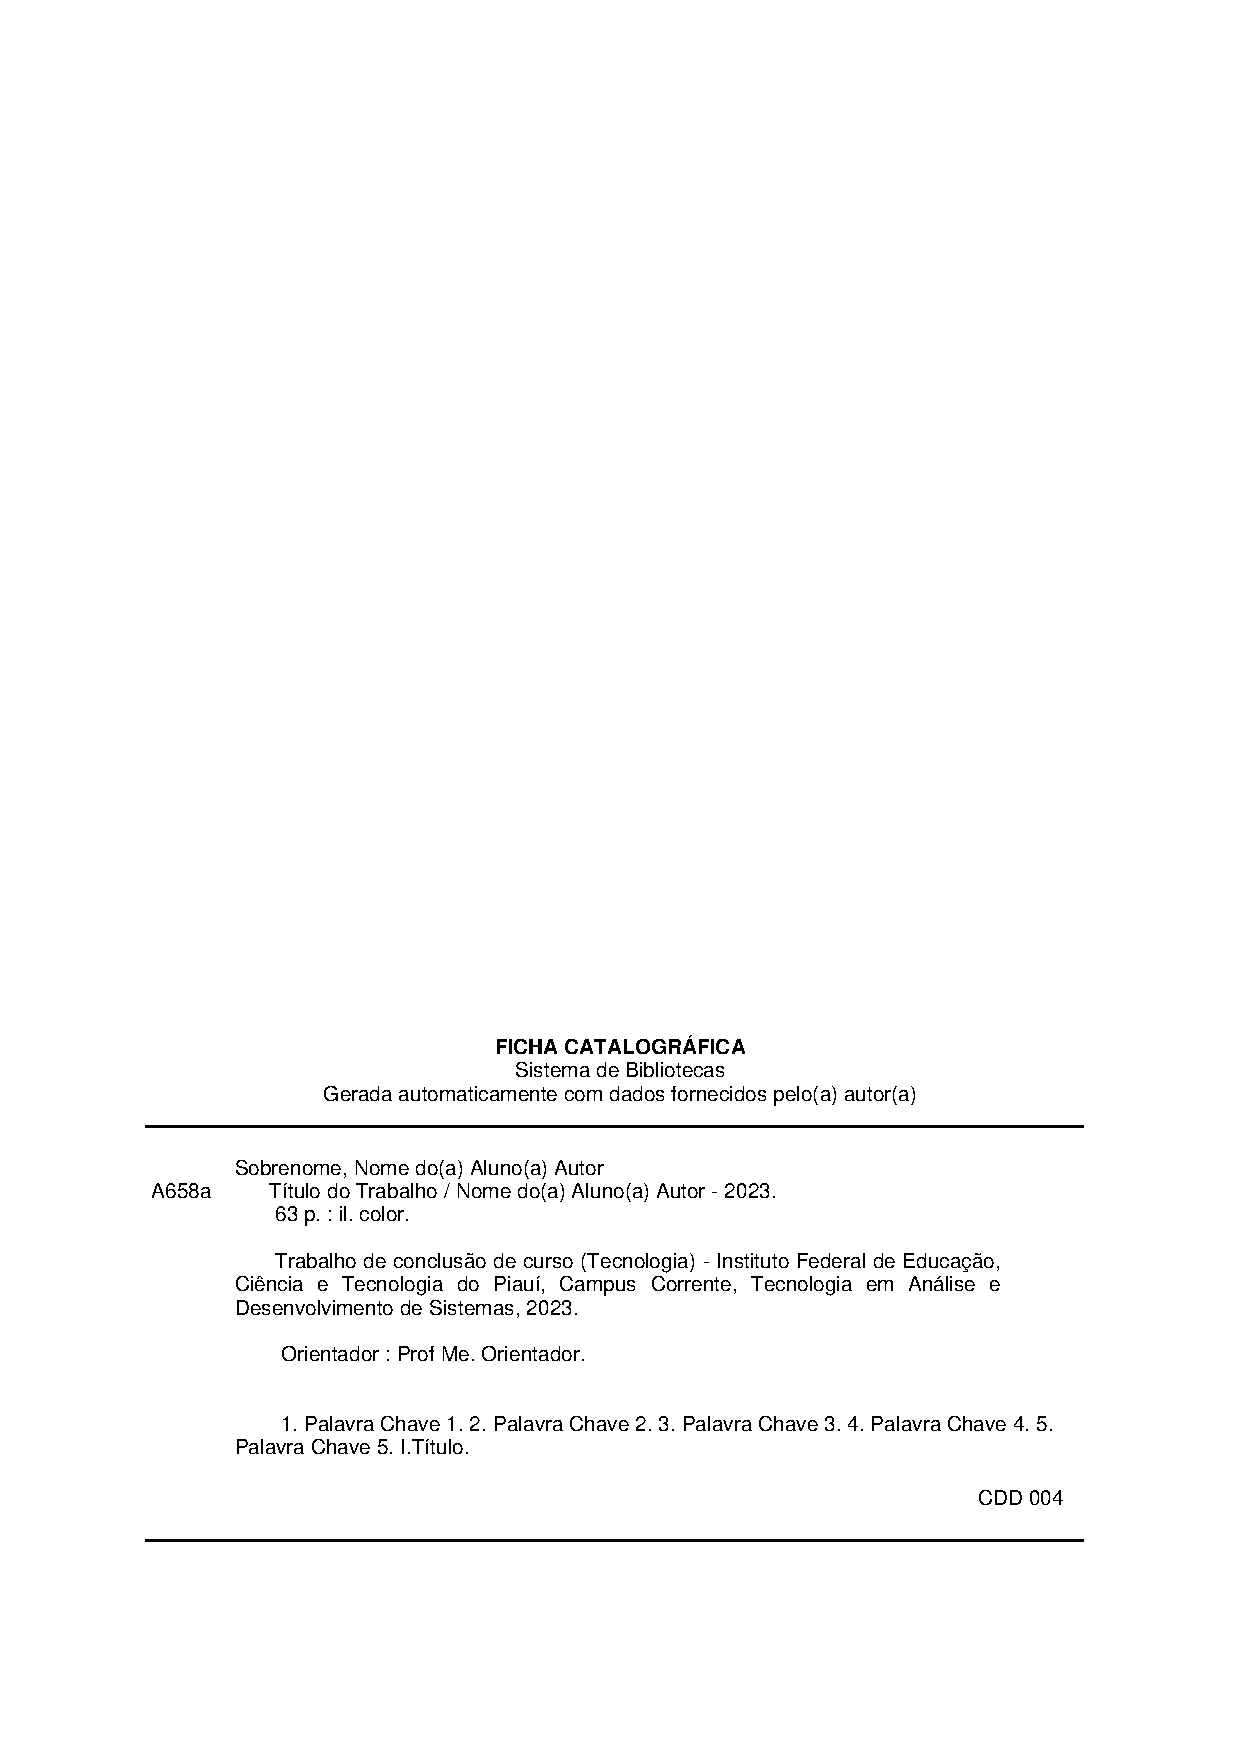
\includepdf{pre-textual/ficha-catalografica.pdf}

%% Caso queira fazer a ficha "tradicional" (este serve apenas como um modelo)
%\begin{fichacatalografica}
%	\sffamily
%	\vspace*{\fill}					% Posição vertical
%	\begin{center}					% Minipage Centralizado
%	\fbox{\begin{minipage}[c][8cm]{13.5cm}		% Largura
%	\small
%	\imprimirautor
%	
%	\hspace{0.5cm} \imprimirtitulo  / \imprimirautor. --
%	\imprimirlocal, \imprimirdata-
%	
%	\hspace{0.5cm} \thelastpage p. : il. (algumas color.) ; 30 cm.\\
%	
%	\hspace{0.5cm} \imprimirorientadorRotulo~\imprimirorientador\\
%	
%	\hspace{0.5cm}
%	\parbox[t]{\textwidth}{\imprimirtipotrabalho~--~\imprimirinstituicao,
%	\imprimirdata.}\\
%	
%	\hspace{0.5cm}
%		1. Palavra-chave1.
%		2. Palavra-chave2.
%		2. Palavra-chave3.
%		I. Orientador.
%		II. Universidade xxx.
%		III. Faculdade de xxx.
%		IV. Título 			
%	\end{minipage}}
%	\end{center}
%\end{fichacatalografica}


%% 03: Errata
%%%% Errata
%\begin{errata}
%Elemento opcional da norma ABNT NBR14724 de 2011. Exemplo:
%
%\vspace{\onelineskip}
%
%FERRIGNO, C. R. A. \textbf{Tratamento de neoplasias ósseas apendiculares com reimplantação de enxerto ósseo autólogo autoclavado associado ao plasma rico em plaquetas}: estudo crítico na cirurgia de preservação de membro em cães. 2011. 128 f. Tese (Livre-Docência) - Faculdade de Medicina Veterinária e Zootecnia, Universidade de São Paulo, São Paulo, 2011.

%% Tabela de exemplo com os erros
%\begin{table}[htb]
%\center
%\footnotesize
%\begin{tabular}{|p{1.4cm}|p{1cm}|p{3cm}|p{3cm}|}
%  \hline
%   \textbf{Folha} & \textbf{Linha}  & \textbf{Onde se lê}  & \textbf{Leia-se}  \\
%    \hline
%    1 & 10 & auto-conclavo & autoconclavo\\
%   \hline
%\end{tabular}
%\end{table}
%
%\end{errata}



%% 04: Folha de Aprovação
%%\imprimirfolhadeaprovacao
%% Use esta se forem 4 membros na banca:
%\imprimirfolhadeaprovacaoduascolunas



%% 05: Dedicatória
%%%% Dedicatória do seu trabalho
\begin{dedicatoria}
	%% Empura o texto a seguir para a parte de baixo da página
	\vspace*{\fill}
    
    %% Alinhado a Direita
    \center
    \begin{flushright}
    	Dedico este trabalho a todos que acreditaram que ele sairia.
    \end{flushright}
    
    %% Descomente a linha seguir para deixar o texto centralizado verticalmente na página
    %% Lembre de comentar o "\begin{}" e "\end{}" acima para centralizar o texto da dedicatória.
	%\vspace*{\fill}
\end{dedicatoria}



%% 06: Agradecimentos
%%%% Agradecimentos
\begin{agradecimentos}
Agradeço a todos os professores e servidores do IFPI do Campus Corrente, pois todos xxxxxxxxxxxxxxxxxxxxxxxxxxxxxxx. Xxxxxxxxxxxxxxxxxxx, que deu todo o apoio necessário para que chegasse até aqui. Agradeço ao meu Deus, que me deu força quando mais precisava.
\end{agradecimentos}



%% 07: Epígrafe
%%%% Epígrafe
%% Uma frase que lhe inspira ou a qual lhe inspirou a fazer este trabalho
\begin{epigrafe}
\vspace*{\fill}
\begin{flushright}
\emph{O que prevemos raramente ocorre; o que 
 \\menos esperamos XXXXXX”. 
  \\ Benjamin Disraeli}
\end{flushright}
\end{epigrafe}



%% 08: Resumo
%%%% Resumo
\begin{resumo}
Apresentação concisa dos pontos relevantes do documento. Deve Informar ao leitor 
finalidades, metodologia, resultados e conclusões do documento, de tal forma que 
este possa, inclusive, dispensar a consulta ao original. Deve-se usar o verbo na voz 
ativa e na terceira pessoa do singular, contendo de 150 a 500 palavras. O resumo 
deve ser composto de uma sequência de frases concisas, afirmativas e não de 
enumeração de tópicos. Recomenda-se o uso de parágrafo único, mesma fonte do 
trabalho, e espaçamento entrelinhas 1,5. Resumo resumo resumo resumo resumo 
resumo resumo resumo resumo resumo resumo resumo resumo resumo resumo 
resumo resumo resumo resumo resumo resumo resumo resumo resumo resumo 
resumo resumo resumo resumo resumo resumo resumo resumo resumo resumo 
resumo ( ASSOCIAÇÃO BRASILEIRA DE NORMAS TÉCNICAS, 2021).
\vspace{\onelineskip}
\noindent

\textbf{Palavras-chaves}: Palavra 1; Palavra 2; 
Palavra 3.
\end{resumo}

%% 09: Abstract/Resumo em língua estrangeira
%%%% Abstract (configurado para língua inglesa)
\begin{resumo}[Abstract]			% Título do Resumo (Abstract = Resumo em inglês)
\begin{otherlanguage*}{english}		% Língua do texto
Elemento obrigatório, com as mesmas características do resumo em língua 
vernácula, digitado em folha separada (em inglês Abstract, em espanhol Resumen, 
em francês Résumé, por exemplo). Abstract abstract abstract abstract abstract 
abstract abstract abstract abstract abstract abstract abstract abstract abstract 
abstract abstract abstract abstract abstract abstract abstract abstract abstract 
abstract abstract abstract abstract abstract abstract abstract abstract abstract 
abstract abstract abstract. ( ASSOCIAÇÃO BRASILEIRA DE NORMAS TÉCNICAS, 2021). 

\vspace{\onelineskip}
\noindent
\textbf{Keywords}: Word 1; Word 2; Word 3.
\end{otherlanguage*}
\end{resumo}

%% Exemplo de resumo em francês
%\begin{resumo}[Résumé]
% \begin{otherlanguage*}{french}
%    Il s'agit d'un résumé en français.
% 
%   \textbf{Mots-clés}: latex. abntex. publication de textes.
% \end{otherlanguage*}
%\end{resumo}

%% Exemplo de resumo em Espanhol
%\begin{resumo}[Resumen]
% \begin{otherlanguage*}{spanish}
%   Este es el resumen en español.
%  
%   \textbf{Palabras clave}: latex. abntex. publicación de textos.
% \end{otherlanguage*}
%\end{resumo}
% ---



%% 10: Lista de Ilustrações
%%%% Lista de Ilustrações
\pdfbookmark[0]{\listfigurename}{lof}
\listoffigures*
\cleardoublepage



%% 11: Lista de Tabelas
%%%% Lista de Tabelas
%\pdfbookmark[0]{\listtablename}{lot}
%\listoftables*
%\cleardoublepage



%% 12: Lista de Abreviaturas e Siglas
%%%% Lista de Siglas
\begin{siglas}
  \item[ABNT] Associação Brasileira de Normas Técnicas
  \item[CRB] Conselho Regional de Biblioteconomia
  \item[IBGE] Instituto Brasileiro de Geografia e Estatística
  \item[IFPI] Instituto Federal de Educação, Ciência e Tecnologia do Piauí
  \item[UFPI] Universidade Federal do Piauí
\end{siglas}



%% 13: Lista de Símbolos
%%%% Lista de Símbolos
%% (esta é apenas uma lista de exemplo)
\begin{simbolos}
  \item [\% ] Porcentagem
  \item [ © ] Copyright
  \item [ ® ] Marca registrada
  \item [ \$ ] Dólar
  \item [ § ] Seção
  \item[$ \Gamma $] Letra grega Gama
  \item[$ \Lambda $] Lambda
  \item[$ \zeta $] Letra grega minúscula zeta
  \item[$ \in $] Pertence
\end{simbolos}



%% 14: Sumário (o asterisco retira o próprio sumário do sumário)
\pdfbookmark[0]{\contentsname}{toc}
\tableofcontents*
\cleardoublepage




  %% Indica que a partir daqui ficarão os elementos textuais (TCC em si)
  \textual

  %% Inclui os capítulos do TCC (parte textual)
  %% %%%%%%%%%%%%%%%%%%%%%%%%%%%%%%%%%%% %%
%% Elementos Textuais (Capítulos)      %%
%% %%%%%%%%%%%%%%%%%%%%%%%%%%%%%%%%%%% %%
\pagestyle{empty} % Remover cabeçalho com titulo dos capítulos
%% Inclua aqui os capítulos que farão parte do TCC
% ----------------------------------------------------------
% Introdução
% ----------------------------------------------------------
\chapter{Introdução}

\section{Objetivos}
\subsection{Objetivo geral}
Analisar o desempenho de aplicativos Android desenvolvidos em React Native, um conjunto de bibliotecas e estruturas na linguagem Javascript, e  Kotlin afim de identificar diferenças em termos de eficiência, uso de recursos e experiência do usuário.
\subsection{Objetivos específicos}
Analisar todo o processo de desenvolvimento do ciclo de vida de uma aplicação nas duas tecnologias, dessa forma, tem-se como objetivos analisar os seguintes pontos:
\begin{description}
	\item[Codificação] Semântica e sintaxe de cada linguagem
	\item[Testes] Facilidade para integração de testes
	\item[Experiência do Usuário] Comportamento do usuário em cada abordagem, incluindo tempo de carregamento e fluidez de navegação
	\item[Manutenção] Capacidade para manutenção e escalabilidade
	\item[Performance] Tempo de resposta e velocidade de execução, comparando os dois métodos de desenvolvimento.
\end{description}
% ----------------------------------------------------------
% Fundamentação Teórica
% ----------------------------------------------------------
\chapter{Fundamentação Teórica}
O desenvolvimento de aplicativos móveis se tornou fundamental na era digital, com um aumento significativo no número de dispositivos móveis em todo o mundo \cite{statista:uso_celular}. Esse crescimento impulsionou o desenvolvimento de tecnologias que otimizam o processo de criação de aplicativos para as duas plataformas móveis mais populares: iOS e Android. No entanto, a criação de aplicativos para múltiplas plataformas apresenta desafios como compatibilidade, desempenho e manutenção de código, o que incentivou a criação de frameworks de desenvolvimento nativo e cross-platform para superar essas barreiras.

\section{Desenvolvimento Nativo}
Desenvolvimento nativo refere-se ao processo de criação de aplicativos usando linguagens e ferramentas específicas para cada sistema operacional. No caso do Android, as principais linguagens são Java e Kotlin, enquanto o iOS utiliza Swift e Objective-C. O desenvolvimento nativo é conhecido por oferecer melhor desempenho e integração com os recursos do dispositivo, pois o código é compilado diretamente para a plataforma de destino.

Por outro lado, o desenvolvimento cross-platform permite que os desenvolvedores escrevam um único código que funcione em múltiplas plataformas. Ferramentas como React Native, Flutter e Xamarin são populares nesse campo. Essa abordagem reduz o tempo e o custo de desenvolvimento, permitindo que equipes lancem produtos rapidamente. No entanto, frameworks cross-platform podem enfrentar limitações em relação ao desempenho e à personalização de interfaces, devido à necessidade de "pontes" para comunicação com componentes nativos.
% ----------------------------------------------------------
% Metodologia
% ----------------------------------------------------------
\chapter{Metodologia}

Bla bla bla metodologia ...
\chapter{Recursos}
%%\input{capitulos/resultados}
%%\input{capitulos/trabalhos-futuros}

  %% Finalizações para o PDF
  \bookmarksetup{startatroot}

  %% Elementos pós-textuais: Referências, Anexos, etc.
  %% %%%%%%%%%%%%%%%%%%%%%%%%%%%%%%%%%%%%%%%%% %%
%% Elementos Pós Textuais
%% ----------------------
%% 
%% Segundo o manual do IFPI, eles devem ser os seguintes (nessa ordem):
%% 1. Referências (obrigatório)
%% 2. Glossário (opcional)
%% 3. Apêndice (opcional)
%% 4. Anexos (opcional)
%% 5. Índices (opcional)
%% %%%%%%%%%%%%%%%%%%%%%%%%%%%%%%%%%%%%%%%%% %%

%% Indica ao LaTeX que a partir deste ponto ficarão os elementos pós-textuais
\postextual

%% 01: Referências bibliográficas
%% Referências bibliográficas

\bibliography{bibliografia}

%% 02: Glossário
%% Glossário
%\glossary

%% 03: Apêndices
%% Apêndices

%\begin{apendicesenv}
%
%%% Imprime uma página indicando o início dos apêndices (opcional, comente para retirar)
%\partapendices
%
%%% Cada Capítulo será um apêndice
%\chapter{Este será o apêndice A}
%Lorem ipsum dolor sit amet, consectetur adipiscing elit. Praesent congue, turpis quis rutrum fringilla, lacus lorem faucibus diam, sit amet viverra urna quam sed metus. Pellentesque quis eros ex. Nullam vel ante rutrum eros placerat egestas. Morbi volutpat sapien elementum tincidunt fringilla. Class aptent taciti sociosqu ad litora torquent per conubia nostra, per inceptos himenaeos. Sed rutrum vestibulum bibendum. Sed tincidunt, magna sit amet tempor tincidunt, turpis neque blandit eros, a tincidunt felis mauris vitae est. Aliquam sit amet placerat risus. Nunc eget est pulvinar est tristique convallis sit amet vel risus. Maecenas turpis nisl, blandit ac porttitor non, ultrices id est. Cras eleifend nulla ut condimentum ullamcorper. Quisque at gravida massa, fringilla varius sapien. Nulla ullamcorper mauris vel ipsum elementum, vel tincidunt ante pretium. Ut iaculis nunc ex, vitae elementum ante efficitur non. Pellentesque venenatis tristique odio, nec volutpat dui dapibus sit amet. Maecenas eu velit at arcu hendrerit sagittis vel a odio.
%
%Nulla gravida metus at gravida ultricies. Nulla auctor id mi id suscipit. Proin vestibulum metus non eros feugiat, ac blandit diam vestibulum. Sed in arcu eget mauris rhoncus semper. Integer dignissim dui quis massa vestibulum, luctus ultrices metus mollis. Sed aliquam leo hendrerit lacus ultricies efficitur. Praesent quis quam sed lorem tincidunt fringilla non interdum odio. Phasellus vel enim mattis, tempor arcu ut, pulvinar est. Sed ut tempus est. Fusce erat nisi, scelerisque quis tellus sit amet, lacinia sagittis libero. Sed ultrices odio ipsum, ut vestibulum nulla auctor in.
%
%
%
%
%
%\chapter{Este será o apêndice B}
%Lorem ipsum dolor sit amet, consectetur adipiscing elit. Integer malesuada elit vel lacus fringilla, in luctus orci finibus. Praesent eget augue et enim luctus cursus ut ac nisl. In lobortis tellus non mauris euismod, tempus hendrerit nisi euismod. Integer id magna sapien. Nunc urna magna, consequat sed vehicula quis, convallis non justo. Aliquam risus dolor, viverra quis dignissim eget, convallis id sapien. Ut id turpis suscipit, mollis quam sed, lacinia lacus. Donec ac nulla dui.
%
%
%\end{apendicesenv}

%% 04: Anexos
%% Anexos
\begin{anexosenv}

%% Imprime uma página indicando o início dos anexos (opcional, comente para retirar)
%\partanexos

% Exemplo de inclusão
% \input{pos-textual/anexo} 
%%\chapter{Avaliação de eficácia comunicativa} \label{anexo:a}
%%\vspace{-2cm}
%%\begin{figure}[H]
	%%\caption*{}
	%%\begin{center}
	    %%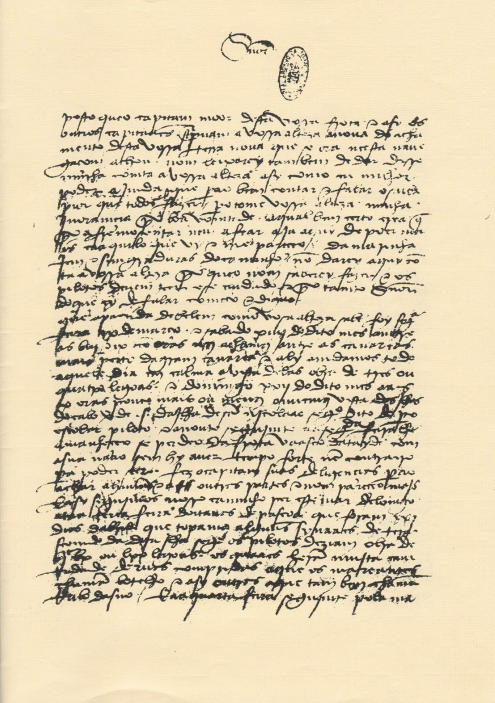
\includegraphics[scale=1.0]{imagens/carta_pero_vaz.png}
	%%\end{center}
	
%%\end{figure}


\end{anexosenv}

%% 05: Índices
%% Índices
%\phantompart \printindex

%% Capa do CD (opcional)
%%% Isso aqui cria a capa do CD, no final do documento :)
\newpage
\thispagestyle{empty}
\begin{center}
\covers[{\vspace{1.5cm} \Large \MakeUppercase{Curso de \imprimirnomedocurso} \\ \vspace{1cm} \textbf{\imprimirautor} \\ \vspace{0.5cm} {TÍTULO: \imprimirtitulo}}]{
	{\vspace{1.5cm} 
\includegraphics[scale=0.25]{imagens/ifpi.pdf} \\ \vspace{1cm} \MakeUppercase{Curso de \imprimirnomedocurso} \\ \vspace{1cm} {\textbf{\imprimirautor}} \\ \vspace{0.3cm} {TÍTULO: \imprimirtitulo} \\ \vspace{1.5cm} \MakeUppercase{\imprimirlocal} \par \imprimirdata}
}{
	\MakeUppercase{\tiny \imprimirtitulo}
}
\end{center}

\end{document}